\section{Loop-Related Directives}
\label{sec:LoopRelatedConstructs}

\subsection{Canonical Loop Form}
\label{subsec:Canonical Loop Form}
\index{canonical loop form}
\begin{ccppspecific}
The loops associated with a loop-associated directive have \emph{canonical loop form} 
if they conform to the following:

\medskip
\nolinenumbers
\renewcommand{\arraystretch}{1.0}
\tablefirsthead{%
    \hline\\[-2ex]
    \multicolumn{2}{l}{\hspace*{-5pt}%
        {\scode{for (}\splc{init-expr}\scode{; }\splc{test-expr}\scode{; }\splc{incr-expr}\scode{) }\splc{structured-block}}}\\[2pt]
    \hline\\[-2ex]
}
\tablehead{%
    \multicolumn{2}{l}{\small\slshape continued from previous page}\\
    \hline\\[-2ex]
}
\tabletail{%
    \hline\\[-2ex]
    \multicolumn{2}{l}{\small\slshape continued on next page}\\
}
\tablelasttail{\hline}
\begin{supertabular}{ p{0.8in} p{4.5in}}
    {\splc{init-expr}} & One of the following:\\
    & {\splc{var}} = {\splc{lb}}\\
    & {\splc{integer-type}} {\splc{var}} = {\splc{lb}}\\
    & {\splc{random-access-iterator-type}} {\splc{var}} = {\splc{lb}}\\
    & {\splc{pointer-type}} {\splc{var}} = {\splc{lb}}\\
    & \\
    {\splc{test-expr}} & One of the following:\\
    & {\splc{var}} {\splc{relational-op}} {\splc{b}}\\
    & {\splc{b}} {\splc{relational-op}} {\splc{var}}\\
    & \\
    {\splc{incr-expr}} & One of the following:\\
    & ++{\splc{var}}\\
    & {\splc{var}}++\\
    & {-} {-} {\splc{var}}\\
    & {\splc{var}} {-} {-}\\
    & {\splc{var}} += {\splc{incr}}\\
    & {\splc{var}} {-} = {\splc{incr}}\\
    & {\splc{var}} = {\splc{var}} + {\splc{incr}}\\
    & {\splc{var}} = {\splc{incr}} + {\splc{var}}\\
    & {\splc{var}} = {\splc{var}} - {\splc{incr}}\\
    & \\
    {\splc{var}} & One of the following:\\
    & \hspace{1.5em}A variable of a signed or unsigned integer type.\\
    & \hspace{1.5em}For C++, a variable of a random access iterator type.\\
    & \hspace{1.5em}For C, a variable of a pointer type.\\
    & This variable must not be modified during the execution of the {\splc{for-loop}}
    other than in {\splc{incr-expr}}. \\
    {\splc{relational-op}} & One of the following:\\
    & {\scode{<}}\\
    & {\scode{<=}}\\
    & {\scode{>}}\\
    & {\scode{>=}}\\
    & {\scode{!=}}\\
    & \\
    {\splc{lb}} and {\splc{b}} & Expressions of a type compatible with the
    type of {\splc{var}} that are loop invariant with respect to the outermost
    associated loop or are one of the following (where {\splc{var-outer}},
    {\splc{a1}}, and {\splc{a2}} have a type compatible with the type of
    {\splc{var}}, {\splc{var-outer}} is {\splc{var}} from an outer associated
    loop, and {\splc{a1}} and {\splc{a2}} are loop invariant integer
    expressions with respect to the outermost loop): \\
    & {\splc{var-outer}} \\
    & {\splc{var-outer}} + {\splc{a2}} \\
    & {\splc{a2}} + {\splc{var-outer}} \\
    & {\splc{var-outer}} - {\splc{a2}} \\
    & {\splc{a2}} - {\splc{var-outer}} \\
    & {\splc{a1}} {*} {\splc{var-outer}} \\
    & {\splc{a1}} {*} {\splc{var-outer}} + {\splc{a2}} \\
    & {\splc{a2}} + {\splc{a1}} {*} {\splc{var-outer}} \\
    & {\splc{a1}} {*} {\splc{var-outer}} - {\splc{a2}} \\
    & {\splc{a2}} - {\splc{a1}} {*} {\splc{var-outer}} \\
    & {\splc{var-outer}} {*} {\splc{a1}} \\
    & {\splc{var-outer}} {*} {\splc{a1}} + {\splc{a2}} \\
    & {\splc{a2}} + {\splc{var-outer}} {*} {\splc{a1}} \\
    & {\splc{var-outer}} {*} {\splc{a1}} - {\splc{a2}} \\
    & {\splc{a2}} - {\splc{var-outer}} {*} {\splc{a1}} \\
    & \\
    {\splc{incr}} & An integer expression that is loop invariant with respect
    to the outermost associated loop.\\
\end{supertabular}
\medskip

\end{ccppspecific}

\begin{fortranspecific}

The loops associated with a loop-associated directive have \emph{canonical loop form} 
if each of them is a \plc{do-loop} that is a \plc{do-construct} or an
\plc{inner-shared-do-construct} as defined by the Fortran standard. If an
\code{end}~\code{do} directive follows a \plc{do-construct} in which several
loop statements share a \code{DO} termination statement, then the directive
can only be specified for the outermost of these \code{DO} statements.

The \plc{do-stmt} for any \plc{do-loop} must conform to the following:

\medskip
\nolinenumbers
\renewcommand{\arraystretch}{1.0}
\tablefirsthead{%
    \hline\\[-2ex]
    \multicolumn{2}{l}{\hspace*{-5pt}%
    {\scode{DO} \splc{[} \splc{label} \splc{]} \splc{var}  \scode{=} \splc{lb} \scode{,} \splc{b} \splc{[} \scode{,} \splc{incr} \splc{]}}}\\[2pt] \hline\\[-2ex]
}
\tablelasttail{\hline}
\begin{supertabular}{ p{0.8in} p{4.5in}}
    {\splc{var}} & A variable of integer type.\\
    & \\

    {\splc{lb}} and {\splc{b}} & Expressions of a type compatible with the
    type of {\splc{var}} that are loop invariant with respect to the outermost
    associated loop or are one of the following (where {\splc{var-outer}},
    {\splc{a1}}, and {\splc{a2}} have a type compatible with the type of
    {\splc{var}}, {\splc{var-outer}} is {\splc{var}} from an outer associated
    loop, and {\splc{a1}} and {\splc{a2}} are loop invariant integer
    expressions with respect to the outermost loop): \\
    & {\splc{var-outer}} \\
    & {\splc{var-outer}} + {\splc{a2}} \\
    & {\splc{a2}} + {\splc{var-outer}} \\
    & {\splc{var-outer}} - {\splc{a2}} \\
    & {\splc{a2}} - {\splc{var-outer}} \\
    & {\splc{a1}} {*} {\splc{var-outer}} \\
    & {\splc{a1}} {*} {\splc{var-outer}} + {\splc{a2}} \\
    & {\splc{a2}} + {\splc{a1}} {*} {\splc{var-outer}} \\
    & {\splc{a1}} {*} {\splc{var-outer}} - {\splc{a2}} \\
    & {\splc{a2}} - {\splc{a1}} {*} {\splc{var-outer}} \\
    & {\splc{var-outer}} {*} {\splc{a1}} \\
    & {\splc{var-outer}} {*} {\splc{a1}} + {\splc{a2}} \\
    & {\splc{a2}} + {\splc{var-outer}} {*} {\splc{a1}} \\
    & {\splc{var-outer}} {*} {\splc{a1}} - {\splc{a2}} \\
    & {\splc{a2}} - {\splc{var-outer}} {*} {\splc{a1}} \\
    & \\

    {\splc{incr}} & An integer expression that is loop invariant with respect
    to the outermost associated loop. If it is not explicitly specified, its value is
    assumed to be 1. \\
\end{supertabular}
\medskip
\end{fortranspecific}


\linenumbers

The canonical form allows the iteration count of all associated loops
to be computed before executing the outermost loop. The \plc{incr} and
\plc{range-expr} are evaluated before executing the loop-associated
construct. If \plc{b} or \plc{lb} is loop invariant with respect to
the outermost associated loop, it is evaluated before executing the
loop-associated construct. If \plc{b} or \plc{lb} is not loop
invariant with respect to the outermost associated loop, \plc{a1}
and/or \plc{a2} are evaluated before executing the loop-associated
construct. The computation is performed for each loop in an integer
type. This type is derived from the type of \plc{var} as follows:

\begin{itemize}
\item If \plc{var} is of an integer type, then the type is the type of \plc{var}.
\end{itemize}        

\begin{cppspecific}
\begin{itemize}
\item If \plc{var} is of a random access iterator type, then the type is the 
      type that would be used by \plc{std::distance} applied to variables of 
      the type of \plc{var}.
\end{itemize}
\end{cppspecific}

\begin{cspecific}
\begin{itemize}
\item If \plc{var} is of a pointer type, then the type is \code{ptrdiff_t}.
\end{itemize}
\end{cspecific}

The behavior is unspecified if any intermediate result required to compute the 
iteration count cannot be represented in the type determined above.

There is no implied synchronization during the evaluation of the \plc{lb}, \plc{b}, 
or \plc{incr} expressions. It is unspecified whether, in what order, or how many 
times any side effects within the \plc{lb}, \plc{b}, or \plc{incr} expressions occur.

\begin{note}
Random access iterators are required to support random access to elements in
constant time. Other iterators are precluded by the restrictions since they can 
take linear time or offer limited functionality. The use of tasks to parallelize 
those cases is therefore advisable.
\end{note}

\begin{cppspecific}

A range-based for loop that is valid in the base language and has a begin value
that satisfies the random access iterator requirement has \emph{canonical loop form}.
Range-based for loops are of the following form:

\scode{for (}\splc{range-decl}\scode{: }\splc{range-expr}\scode{) }\splc{structured-block}


The \plc{begin-expr} and \plc{end-expr} expressions are derived from
\plc{range-expr} by the base language and assigned to variables to which this
specification refers as \code{__begin} and \code{__end} respectively.  Both
\code{__begin} and \code{__end} are privatized.  For the purpose of the rest of
the standard \code{__begin} is the iteration variable of the range-for loop.

\end{cppspecific}

\restrictions
The following restrictions also apply:

\begin{ccppspecific}
\begin{itemize}
\item If \plc{test-expr} is of the form \plc{var} \plc{relational-op}
      \plc{b} and \plc{relational-op} is < or <= then \plc{incr-expr} 
      must cause \plc{var} to increase on each iteration of the loop. 
      If \plc{test-expr} is of the form \plc{var} \plc{relational-op} 
      \plc{b} and \plc{relational-op} is > or >= then \plc{incr-expr} 
      must cause \plc{var} to decrease on each iteration of the loop.
\item If \plc{test-expr} is of the form \plc{b} \plc{relational-op}
      \plc{var} and \plc{relational-op} is < or <= then \plc{incr-expr} 
      must cause \plc{var} to decrease on each iteration of the loop. 
      If \plc{test-expr} is of the form \plc{b} \plc{relational-op} 
      \plc{var} and \plc{relational-op} is > or >= then \plc{incr-expr} 
      must cause \plc{var} to increase on each iteration of the loop.
\item If \plc{test-expr} is of the form \plc{b} != \plc{var} or
      \plc{var} != \plc{b} then \plc{incr-expr} must cause \plc{var}
      either to increase on each iteration of the loop or to decrease on
      each iteration of the loop.
\item If \plc{relational-op} is != and \plc{incr-expr} is of the
      form that has \plc{incr} then \plc{incr} must be a constant 
      expression and evaluate to -1 or 1.
\end{itemize}
\end{ccppspecific}

\begin{cppspecific}
\begin{itemize}
\item In the \code{simd} construct the only random access iterator types
      that are allowed for \plc{var} are pointer types.
\item The \plc{range-expr} of a range-for loop must be loop invariant
      with respect to the outermost associated loop, and must not reference
      iteration variables of any associated loops.
\item The loops associated with an ordered clause with a parameter may not
      include range-for loops.
\end{itemize}
\end{cppspecific}

\begin{itemize}
\item The \plc{b}, \plc{lb}, \plc{incr}, and \plc{range-expr} expressions
      may not reference any \plc{var} or member of the \plc{range-decl} of
      any enclosed associated loop.
\item For any associated loop where the \plc{b} or \plc{lb} expression is not loop
      invariant with respect to the outermost loop, the \plc{var-outer} that
      appears in the expression may not have a random access iterator type.
\item For any associated loop where \plc{b} or \plc{lb} is not loop invariant
      with respect to the outermost loop, the expression $\plc{b}-\plc{lb}$
      will have the form $\plc{c}*\plc{var-outer}+\plc{d}$, where \plc{c} and
      \plc{d} are loop invariant integer expressions. Let \plc{incr-outer} be
      the \plc{incr} expression of the outer loop referred to by \plc{var-outer}.  
      The value of $\plc{c}*\plc{incr-outer} \mod \plc{incr}$ must be 0.
\end{itemize}

\begin{crossrefs}
\item \code{simd} construct, see \specref{subsubsec:simd Construct}.

\item \code{lastprivate} clause, see \specref{subsubsec:lastprivate clause}.

\item \code{linear} clause, see \specref{subsubsec:linear clause}.
\end{crossrefs}



\subsection{Worksharing-Loop Construct}
\label{subsec:Worksharing-Loop Construct}
\index{worksharing-loop construct}
\index{constructs!worksharing-loop construct}
\index{constructs!do@{\code{do} \emph{Fortran}}}
\index{do@{\code{do}, \emph{Fortran}}}
\index{for@{\code{for}, \emph{C/C++}}}
\index{constructs!for@{\code{for}, \emph{C/C++}}}
\summary
The worksharing-loop construct specifies that the iterations of one or more 
associated loops will be executed in parallel by threads in the team in the 
context of their implicit tasks. The iterations are distributed across threads 
that already exist in the team that is executing the \code{parallel} region 
to which the worksharing-loop region binds.

\syntax
\begin{ccppspecific}
The syntax of the worksharing-loop construct is as follows:

\begin{ompcPragma}
#pragma omp for \plc{[clause[ [},\plc{] clause] ... ] new-line}
    \plc{for-loops}
\end{ompcPragma}

where clause is one of the following:
\index{clauses!collapse@{\code{collapse}}}

{}
\begin{indentedcodelist}
private(\plc{list})
firstprivate(\plc{list})
lastprivate(\plc{[ lastprivate-modifier}:\plc{] list})
linear(\plc{list[ }:\plc{ linear-step]})
reduction(\plc{[ reduction-modifier},\plc{]reduction-identifier }:\plc{ list})
schedule(\plc{[modifier [}, \plc{modifier]}:\plc{]kind[},\plc{ chunk_size]})
collapse(\plc{n})
ordered\plc{[}(\plc{n})\plc{]}
nowait
allocate(\plc{[allocator :]}\plc{list})
order(concurrent)
\end{indentedcodelist}

The \code{for} directive places restrictions on the structure of all associated 
\plc{for-loops}. Specifically, all associated \plc{for-loops} must have 
\emph{canonical loop form} (see \specref{subsec:Canonical Loop Form}).
\end{ccppspecific}

\begin{fortranspecific}
The syntax of the worksharing-loop construct is as follows:

\begin{ompfPragma}
!$omp do \plc{[clause[ [},\plc{] clause] ... ]}
   \plc{do-loops}
\textsl{[}!$omp end do \textsl{[}nowait\textsl{]]}
\end{ompfPragma}

where \plc{clause} is one of the following:

{}
\begin{indentedcodelist}
private(\plc{list})
firstprivate(\plc{list})
lastprivate(\plc{[ lastprivate-modifier}:\plc{] list})
linear(\plc{list[ }:\plc{ linear-step]})
reduction(\plc{[ reduction-modifier},\plc{]reduction-identifier }:\plc{ list})
schedule(\plc{[modifier [}, \plc{modifier]}:\plc{]kind[},\plc{ chunk_size]})
collapse(\plc{n})
ordered\plc{[}(\plc{n})\plc{]}
allocate(\plc{[allocator :]}\plc{list})
order(concurrent)
\end{indentedcodelist}

If an \code{end}~\code{do} directive is not specified, an \code{end}~\code{do} 
directive is assumed at the end of the \plc{do-loops}.

The \code{do} directive places restrictions on the structure of all
associated \plc{do-loops}.  Specifically, all associated \plc{do-loops} must
have \emph{canonical loop form} (see \specref{subsec:Canonical Loop Form}).

\end{fortranspecific}

\binding
The binding thread set for a worksharing-loop region is the current team. A
worksharing-loop region binds to the innermost enclosing \code{parallel} region. 
Only the threads of the team executing the binding \code{parallel} region 
participate in the execution of the loop iterations and the implied barrier 
of the worksharing-loop region if the barrier is not eliminated by a 
\code{nowait} clause.

\descr
The worksharing-loop construct is associated with a loop nest that consists
of one or more loops that follow the directive.

There is an implicit barrier at the end of a worksharing-loop construct 
unless a \code{nowait} clause is specified.

\index{clauses!collapse@{\code{collapse}}}
The \code{collapse} clause may be used to specify how many loops are
associated with the worksharing-loop construct. The parameter of the \code{collapse}
clause must be a constant positive integer expression. If a \code{collapse}
clause is specified with a parameter value greater than 1, then the
iterations of the associated loops to which the clause applies are collapsed
into one larger iteration space that is then divided according
to the \code{schedule} clause. The sequential execution of the iterations
in these associated loops determines the order of the iterations in the
collapsed iteration space. If no \code{collapse} clause is present or its
parameter is 1, the only loop that is associated with the worksharing-loop construct
for the purposes of determining how the iteration space is divided according
to the \code{schedule} clause is the one that immediately follows the
worksharing-loop directive.

If more than one loop is associated with the worksharing-loop construct then the
number of times that any intervening code between any two associated
loops will be executed is unspecified but will be at least once per
iteration of the loop enclosing the intervening code and at most once
per iteration of the innermost loop associated with the construct. If the
iteration count of any loop that is associated with the
worksharing-loop construct is zero and that loop does not enclose the
intervening code, the behavior is unspecified.

The integer type (or kind, for Fortran) used to compute the iteration count
for the collapsed loop is implementation defined.

\index{clauses!schedule@{\code{schedule}}} A worksharing-loop has
logical iterations numbered 0,1,...,N-1 where N is the number of loop
iterations, and the logical numbering denotes the sequence in which
the iterations would be executed if a set of associated loop(s) were
executed sequentially.  At the beginning of each logical iteration,
the loop iteration variable of each associated loop has the value that
it would have if the set of the associated loop(s) were executed
sequentially.  The \code{schedule} clause specifies how iterations of
these associated loops are divided into contiguous non-empty subsets,
called chunks, and how these chunks are distributed among threads of
the team. Each thread executes its assigned chunk(s) in the context of
its implicit task.  The iterations of a given chunk are executed in
sequential order by the assigned thread.  The \plc{chunk_size}
expression is evaluated using the original list items of any variables
that are made private in the worksharing-loop construct. It is unspecified
whether, in what order, or how many times, any side effects of the
evaluation of this expression occur. The use of a variable in a
\code{schedule} clause expression of a worksharing-loop construct causes an
implicit reference to the variable in all enclosing constructs.

Different worksharing-loop regions with the same schedule and iteration count, 
even if they occur in the same parallel region, can distribute iterations among
threads differently. The only exception is for the \code{static} schedule
as specified in Table~\ref{tab:Schedule-Values}. Programs that depend
on which thread executes a particular iteration under any other circumstances
are non-conforming.

See \specref{subsubsec:Determining the Schedule of a Worksharing-Loop}
for details of how the schedule for a worksharing-loop region is
determined.

The schedule \plc{kind} can be one of those specified in
Table~\ref{tab:Schedule-Values}.

The schedule \plc{modifier} can be one of those specified in
Table~\ref{tab:Schedule Clause Modifier Values}. If the
\code{static} schedule kind is specified or if the \code{ordered}
clause is specified, and if the \code{nonmonotonic} modifier is
not specified, the effect is as if the \code{monotonic} modifier
is specified. Otherwise, unless the \code{monotonic} modifier is
specified, the effect is as if the \code{nonmonotonic} modifier
is specified.
If a \code{schedule} clause specifies a modifier then that modifier overrides
any modifier that is specified in the \plc{run-sched-var} ICV.

The \code{ordered} clause with the parameter may also be used to specify
how many loops are associated with the worksharing-loop construct. The parameter of
the \code{ordered} clause must be a constant positive integer expression
if specified. The parameter of the \code{ordered} clause does not
affect how the logical iteration space is then divided. If an \code{ordered}
clause with the parameter is specified for the worksharing-loop construct, then those
associated loops form a \emph{doacross loop nest}.

If the value of the parameter in the \code{collapse} or \code{ordered}
clause is larger than the number of nested loops following the construct,
the behavior is unspecified.

If an \code{order(concurrent)} clause is present, then after assigning the
iterations of the associated loops to their respective threads, as specified in
Table \ref{tab:Schedule-Values}, the iterations may be executed in any order,
including concurrently.


\nolinenumbers

\tablefirsthead{%
\hline\\[-3ex]
}
\tablehead{%
\multicolumn{2}{l}{\small\slshape table continued from previous page}\\
\hline\\[-3ex]
}
\tabletail{%
\hline\\[-4ex]
\multicolumn{2}{l}{\small\slshape table continued on next page}\\
}
\tablelasttail{\hline}
\tablecaption{\code{schedule} Clause \plc{kind} Values\label{tab:Schedule-Values}}
\begin{supertabular}{ p{0.8in} p{4.3in} }

{\scode{static}} & When \splc{kind} is \index{static@{{\scode{static}}}}\scode{static},
                   iterations are divided into chunks of size
                   {\splc{chunk_size}}, and the chunks are assigned to the 
                   threads in the team in a round-robin fashion in the order 
                   of the thread number. Each chunk contains {\splc{chunk_size}} 
                   iterations, except for the chunk that contains the sequentially 
                   last iteration, which may have fewer iterations.\\

                 & When no {\splc{chunk_size}} is specified, the iteration space is 
                   divided into chunks that are approximately equal in size, and at 
                   most one chunk is distributed to each thread. The size of the 
                   chunks is unspecified in this case.\\

                 & A compliant implementation of the {\scode{static}} schedule must 
                   ensure that the same assignment of logical iteration numbers to
                   threads will be used in two worksharing-loop regions if the 
                   following conditions are satisfied: 1) both worksharing-loop 
                   regions have the same number of loop iterations, 2) both 
                   worksharing-loop regions have the same value of {\splc{chunk_size}} 
                   specified, or both worksharing-loop regions have no 
                   {\splc{chunk_size}} specified, 3) both worksharing-loop regions 
                   bind to the same parallel region, and 4) neither loop is
                   associated with a SIMD construct. A data dependence between the 
                   same logical iterations in two such loops is guaranteed to be 
                   satisfied allowing safe use of the {\scode{nowait}} clause.\\

{\scode{dynamic}} & When \splc{kind} is \index{dynamic@{{\scode{dynamic}}}}\scode{dynamic},
                    the iterations are distributed to threads in the team
                    in chunks. Each thread executes a chunk of iterations, then 
                    requests another chunk, until no chunks remain to be distributed. \\

                  & Each chunk contains {\splc{chunk_size}} iterations, except for
                    the chunk that contains the sequentially last iteration, which 
                    may have fewer iterations.\\

                  & When no {\splc{chunk_size}} is specified, it defaults to 1.\\

{\scode{guided}} & When \splc{kind} is \index{guided@{{\scode{guided}}}}\scode{guided},
                   the iterations are assigned to threads in the team
                   in chunks. Each thread executes a chunk of iterations, then 
                   requests another chunk, until no chunks remain to be assigned.\\

                 & For a {\splc{chunk_size}} of 1, the size of each chunk is 
                   proportional to the number of unassigned iterations divided by 
                   the number of threads in the team, decreasing to 1. For a 
                   {\splc{chunk_size}} with value $k$ (greater than 1), the
                   size of each chunk is determined in the same way, with the 
                   restriction that the chunks do not contain fewer than $k$ 
                   iterations (except for the chunk that contains the sequentially 
                   last iteration, which may have fewer than $k$ iterations). \\

                 & When no {\splc{chunk_size}} is specified, it defaults to 1.\\

{\scode{auto}} & When \splc{kind} is \index{auto@{{\scode{auto}}}}\scode{auto},
                 the decision regarding scheduling is delegated to the
                 compiler and/or runtime system. The programmer gives the
                 implementation the freedom to choose any possible mapping of
                 iterations to threads in the team.\\

{\scode{runtime}} & When \splc{kind} is \index{runtime@{{\scode{runtime}}}}\scode{runtime},
                    the decision regarding scheduling is deferred until run
                    time, and the schedule and chunk size are taken from the
                    {\splc{run-sched-var}} ICV. If the ICV is set to
                    {\scode{auto}}, the schedule is implementation defined.\\
\end{supertabular}

\linenumbers
\bigskip\bigskip


\begin{note}
For a team of $p$ threads and a loop of $n$ iterations, let $\blceil n/p \brceil$ 
be the integer $q$ that satisfies $n = p*q - r$, with $0 <= r < p$. One compliant 
implementation of the \code{static} schedule (with no specified \plc{chunk_size}) 
would behave as though \plc{chunk_size} had been specified with value $q$. Another 
compliant implementation would assign $q$ iterations to the first $p-r$ threads, 
and $q-1$ iterations to the remaining $r$ threads. This illustrates why a
conforming program must not rely on the details of a particular implementation.

A compliant implementation of the \code{guided} schedule with a \plc{chunk_size} 
value of $k$ would assign $q = \blceil n/p \brceil$ iterations to the first 
available thread and set $n$ to the larger of $n-q$ and $p*k$. It would then 
repeat this process until $q$ is greater than or equal to the number of remaining 
iterations, at which time the remaining iterations form the final
chunk. Another compliant implementation could use the same method, except with
$q = \blceil n/(2p) \brceil$, and set $n$ to the larger of $n-q$ and $2*p*k$.
\end{note}


\nolinenumbers

\tablefirsthead{%
\hline\\[-3ex]
}
\tablehead{%
\multicolumn{2}{l}{\small\slshape table continued from previous page}\\
\hline\\[-3ex]
}
\tabletail{%
\hline\\[-4ex]
\multicolumn{2}{l}{\small\slshape table continued on next page}\\
}
\tablelasttail{\hline}
\tablecaption{\code{schedule} Clause \plc{modifier} Values\label{tab:Schedule Clause Modifier Values}}
%% 
\begin{supertabular}{ p{1in} p{4.1in} }
{\scode{monotonic}} & When the {\scode{monotonic}} modifier is specified then 
                      each thread executes the chunks that it is assigned in 
                      increasing logical iteration order.\\
{\scode{nonmonotonic}} & When the {\scode{nonmonotonic}} modifier is specified 
                         then chunks are assigned to threads in any order and 
                         the behavior of an application that depends on any 
                         execution order of the chunks is unspecified.\\
{\scode{simd}} & When the {\scode{simd}} modifier is specified and the loop 
                 is associated with a SIMD construct, the {\splc{chunk_size}} 
                 for all chunks except the first and last chunks  is  
                 $new\_chunk\_size = \blceil chunk\_size / simd\_width \brceil * simd\_width $ 
                 where {\splc{simd_width}} is an implementation-defined value. 
                 The first chunk will have at least {\splc{new_chunk_size}} 
                 iterations except if it is also the last chunk. The last 
                 chunk may have fewer iterations than {\splc{new_chunk_size}}. 
                 If the {\scode{simd}} modifier is specified and the loop is 
                 not associated  with a SIMD construct, the modifier is ignored.\\
\end{supertabular}
\linenumbers
\medskip

\events
The \plc{ws-loop-begin} event occurs after an implicit task encounters a
worksharing-loop construct but before the task starts execution of the structured
block of the worksharing-loop region.

The \plc{ws-loop-end} event occurs after a worksharing-loop region finishes
execution but before resuming execution of the encountering task.

The \plc{ws-loop-iteration-begin} event occurs once for each iteration of a
worksharing-loop before the iteration is executed by an implicit task.

\tools
A thread dispatches a registered \code{ompt_callback_work} callback with
\code{ompt_scope_begin} as its \plc{endpoint} argument and \code{work_loop}
as its \plc{wstype} argument for each occurrence of a \plc{ws-loop-begin}
event in that thread. Similarly, a thread dispatches a registered
\code{ompt_callback_work} callback with \code{ompt_scope_end} as its
\plc{endpoint} argument and \code{work_loop} as its \plc{wstype} argument
for each occurrence of a \plc{ws-loop-end} event in that thread. The callbacks
occur in the context of the implicit task. The callbacks have type
signature \code{ompt_callback_work_t}.

A thread dispatches a registered \code{ompt_callback_dispatch}
callback for each occurrence of a \plc{ws-loop-iteration-begin} 
event in that thread. The callback occurs in the
context of the implicit task.  The callback has type signature
\code{ompt_callback_dispatch_t}. 

\restrictions
Restrictions to the worksharing-loop construct are as follows:

\begin{itemize}
\item No OpenMP directive may appear in the region between any associated loops.
\item If a \code{collapse} clause is specified, exactly one loop must
      occur in the region at each nesting level up to the number of loops
      specified by the parameter of the \code{collapse} clause.
\item If the \code{ordered} clause is present, all loops associated
      with the construct must be perfectly nested; that is there must be
      no intervening code between any two loops.
\item If a \code{reduction} clause with the \code{inscan} modifier is
      specified, neither the \code{ordered} nor \code{schedule} clause
      may appear on the worksharing-loop directive.
\item The values of the loop control expressions of the loops associated with
      the worksharing-loop construct must be the same for all threads in the team.
\item Only one \code{schedule} clause can appear on a worksharing-loop directive.
\item The \code{schedule} clause must not appear on the worksharing-loop
      directive  if the associated loop(s) form a non-rectangular loop nest.
\item The \code{ordered} clause must not appear on the worksharing-loop directive 
      if the associated loop(s) form a non-rectangular loop nest.
\item Only one \code{collapse} clause can appear on a worksharing-loop directive.
\item \plc{chunk_size} must be a loop invariant integer expression with a 
      positive value.
\item The value of the \plc{chunk_size} expression must be the same for all 
      threads in the team.
\item The value of the \plc{run-sched-var} ICV must be the same for all 
      threads in the team.
\item When \code{schedule(runtime)} or \code{schedule(auto)} is specified, 
      \plc{chunk_size} must not be specified.
\item A \plc{modifier} may not be specified on a \code{linear} clause.
\item Only one \code{ordered} clause can appear on a worksharing-loop directive.
\item The \code{ordered} clause must be present on the worksharing-loop 
      construct if any \code{ordered} region ever binds to a worksharing-loop 
      region arising from the worksharing-loop construct.
\item The \code{nonmonotonic} modifier cannot be specified if an \code{ordered} 
      clause is specified.
\item Either the \code{monotonic} modifier or the \code{nonmonotonic} modifier 
      can be specified but not both.
\item The loop iteration variable may not appear in a \code{threadprivate} directive.
\item If both the \code{collapse} and \code{ordered} clause with a parameter 
      are specified, the parameter of the \code{ordered} clause must be greater 
      than or equal to the parameter of the \code{collapse} clause.
\item A \code{linear} clause or an \code{ordered} clause with a parameter can
      be specified on a worksharing-loop directive but not both.
\item If an \code{order(concurrent)} clause is present, all restrictions from
      the \code{loop} construct with an \code{order(concurrent)} clause also apply.
\item If an \code{order(concurrent)} clause is present, an \code{ordered}
      clause may not appear on the same directive.
\end{itemize}

\begin{ccppspecific}
\begin{itemize}
\item The associated \plc{for-loops} must be structured blocks.
\item Only an iteration of the innermost associated loop may be curtailed 
      by a \code{continue} statement.
\item No statement can branch to any associated \code{for} statement.
\item Only one \code{nowait} clause can appear on a \code{for} directive.
\item A throw executed inside a worksharing-loop region must cause execution 
      to resume within the same iteration of the worksharing-loop region, 
      and the same thread that threw the exception must catch it.
\end{itemize}
\end{ccppspecific}

\begin{fortranspecific}
\begin{itemize}
\item The associated \plc{do-loops} must be structured blocks.
\item Only an iteration of the innermost associated loop may be curtailed 
      by a \code{CYCLE} statement.
\item No statement in the associated loops other than the \code{DO} statements 
      can cause a branch out of the loops.
\item The \plc{do-loop} iteration variable must be of type integer.
\item The \plc{do-loop} cannot be a \code{DO WHILE} or a \code{DO} loop 
      without loop control.
\end{itemize}
\end{fortranspecific}

\begin{crossrefs}
\item \code{order(concurrent)} clause, see \specref{subsec:loop Construct}.

\item \code{ordered} construct, see
\specref{subsec:ordered Construct}.

\item \code{depend} clause, see
\specref{subsec:depend Clause}.

\item \code{private}, \code{firstprivate}, \code{lastprivate}, \code{linear}, 
and \code{reduction} clauses, see \specref{subsec:Data-Sharing Attribute Clauses}.

\item \code{ompt_scope_begin} and \code{ompt_scope_end}, see
  \specref{sec:ompt_scope_endpoint_t}.

\item \code{ompt_work_loop}, see \specref{sec:ompt_work_t}.

\item \code{ompt_callback_work_t}, see
\specref{sec:ompt_callback_work_t}.

\item \code{OMP_SCHEDULE} environment variable, see
\specref{sec:OMP_SCHEDULE}.
\end{crossrefs}



% Figure 2-1: The process for editing a .dia diagram is:
%    1. Use dia to edit the .dia file
%    2. Export to a .tex file
%    3. Edit the .tex file and manually add the \code{} and \plc{} markup.

\begin{figure}[h]
\begin{quote} % to indent the diagram
% Graphic for TeX using PGF
% Title: worksharing-schedule-loop.dia
% Creator: Dia v0.97.2
% CreationDate: Wed Mar 12 03:33:08 2014
% For: dm
% \usepackage{tikz}
% The following commands are not supported in PSTricks at present
% We define them conditionally, so when they are implemented,
% this pgf file will use them.
\ifx\du\undefined
  \newlength{\du}
\fi
\setlength{\du}{15\unitlength}
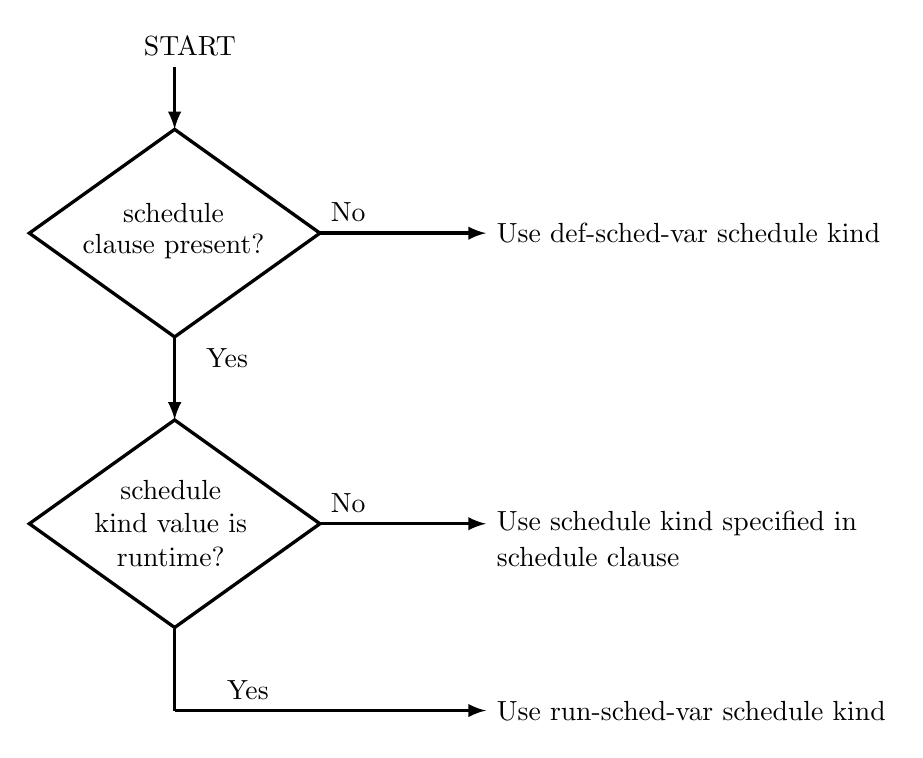
\begin{tikzpicture}
\pgftransformxscale{1.000000}
\pgftransformyscale{-1.000000}
\definecolor{dialinecolor}{rgb}{0.000000, 0.000000, 0.000000}
\pgfsetstrokecolor{dialinecolor}
\definecolor{dialinecolor}{rgb}{1.000000, 1.000000, 1.000000}
\pgfsetfillcolor{dialinecolor}
\definecolor{dialinecolor}{rgb}{1.000000, 1.000000, 1.000000}
\pgfsetfillcolor{dialinecolor}
\fill (18.500000\du,7.000000\du)--(22.000000\du,9.500000\du)--(18.500000\du,12.000000\du)--(15.000000\du,9.500000\du)--cycle;
\pgfsetlinewidth{0.080000\du}
\pgfsetdash{}{0pt}
\pgfsetdash{}{0pt}
\pgfsetmiterjoin
\definecolor{dialinecolor}{rgb}{0.000000, 0.000000, 0.000000}
\pgfsetstrokecolor{dialinecolor}
\draw (18.500000\du,7.000000\du)--(22.000000\du,9.500000\du)--(18.500000\du,12.000000\du)--(15.000000\du,9.500000\du)--cycle;
% setfont left to latex
\definecolor{dialinecolor}{rgb}{0.000000, 0.000000, 0.000000}
\pgfsetstrokecolor{dialinecolor}
\node at (18.500000\du,9.695000\du){};
\pgfsetlinewidth{0.080000\du}
\pgfsetdash{}{0pt}
\pgfsetdash{}{0pt}
\pgfsetbuttcap
{
\definecolor{dialinecolor}{rgb}{0.000000, 0.000000, 0.000000}
\pgfsetfillcolor{dialinecolor}
% was here!!!
\pgfsetarrowsend{latex}
\definecolor{dialinecolor}{rgb}{0.000000, 0.000000, 0.000000}
\pgfsetstrokecolor{dialinecolor}
\draw (18.500000\du,12.000000\du)--(18.500000\du,14.000000\du);
}
\pgfsetlinewidth{0.080000\du}
\pgfsetdash{}{0pt}
\pgfsetdash{}{0pt}
\pgfsetbuttcap
{
\definecolor{dialinecolor}{rgb}{0.000000, 0.000000, 0.000000}
\pgfsetfillcolor{dialinecolor}
% was here!!!
\pgfsetarrowsend{latex}
\definecolor{dialinecolor}{rgb}{0.000000, 0.000000, 0.000000}
\pgfsetstrokecolor{dialinecolor}
\draw (22.000000\du,16.500000\du)--(26.000000\du,16.500000\du);
}
% setfont left to latex
\definecolor{dialinecolor}{rgb}{0.000000, 0.000000, 0.000000}
\pgfsetstrokecolor{dialinecolor}
\node[anchor=west] at (20.000000\du,10.000000\du){};
\pgfsetlinewidth{0.080000\du}
\pgfsetdash{}{0pt}
\pgfsetdash{}{0pt}
\pgfsetbuttcap
{
\definecolor{dialinecolor}{rgb}{0.000000, 0.000000, 0.000000}
\pgfsetfillcolor{dialinecolor}
% was here!!!
\pgfsetarrowsend{latex}
\definecolor{dialinecolor}{rgb}{0.000000, 0.000000, 0.000000}
\pgfsetstrokecolor{dialinecolor}
\draw (18.500000\du,5.500000\du)--(18.500000\du,7.000000\du);
}
% setfont left to latex
\definecolor{dialinecolor}{rgb}{0.000000, 0.000000, 0.000000}
\pgfsetstrokecolor{dialinecolor}
\node[anchor=west] at (31.000000\du,12.000000\du){};
\definecolor{dialinecolor}{rgb}{1.000000, 1.000000, 1.000000}
\pgfsetfillcolor{dialinecolor}
\fill (18.500000\du,14.000000\du)--(22.000000\du,16.500000\du)--(18.500000\du,19.000000\du)--(15.000000\du,16.500000\du)--cycle;
\pgfsetlinewidth{0.080000\du}
\pgfsetdash{}{0pt}
\pgfsetdash{}{0pt}
\pgfsetmiterjoin
\definecolor{dialinecolor}{rgb}{0.000000, 0.000000, 0.000000}
\pgfsetstrokecolor{dialinecolor}
\draw (18.500000\du,14.000000\du)--(22.000000\du,16.500000\du)--(18.500000\du,19.000000\du)--(15.000000\du,16.500000\du)--cycle;
% setfont left to latex
\definecolor{dialinecolor}{rgb}{0.000000, 0.000000, 0.000000}
\pgfsetstrokecolor{dialinecolor}
\node at (18.500000\du,16.695000\du){};
\pgfsetlinewidth{0.080000\du}
\pgfsetdash{}{0pt}
\pgfsetdash{}{0pt}
\pgfsetbuttcap
{
\definecolor{dialinecolor}{rgb}{0.000000, 0.000000, 0.000000}
\pgfsetfillcolor{dialinecolor}
% was here!!!
\pgfsetarrowsend{latex}
\definecolor{dialinecolor}{rgb}{0.000000, 0.000000, 0.000000}
\pgfsetstrokecolor{dialinecolor}
\draw (22.000000\du,9.500000\du)--(26.000000\du,9.500000\du);
}
\pgfsetlinewidth{0.080000\du}
\pgfsetdash{}{0pt}
\pgfsetdash{}{0pt}
\pgfsetbuttcap
{
\definecolor{dialinecolor}{rgb}{0.000000, 0.000000, 0.000000}
\pgfsetfillcolor{dialinecolor}
% was here!!!
\definecolor{dialinecolor}{rgb}{0.000000, 0.000000, 0.000000}
\pgfsetstrokecolor{dialinecolor}
\draw (18.500000\du,19.040000\du)--(18.500000\du,21.000000\du);
}
\pgfsetlinewidth{0.080000\du}
\pgfsetdash{}{0pt}
\pgfsetdash{}{0pt}
\pgfsetbuttcap
{
\definecolor{dialinecolor}{rgb}{0.000000, 0.000000, 0.000000}
\pgfsetfillcolor{dialinecolor}
% was here!!!
\pgfsetarrowsend{latex}
\definecolor{dialinecolor}{rgb}{0.000000, 0.000000, 0.000000}
\pgfsetstrokecolor{dialinecolor}
\draw (18.500000\du,21.000000\du)--(26.000000\du,21.000000\du);
}
% setfont left to latex
\definecolor{dialinecolor}{rgb}{0.000000, 0.000000, 0.000000}
\pgfsetstrokecolor{dialinecolor}
\node[anchor=west] at (17.500000\du,5.000000\du){START};
% setfont left to latex
\definecolor{dialinecolor}{rgb}{0.000000, 0.000000, 0.000000}
\pgfsetstrokecolor{dialinecolor}
\node at (18.471967\du,9.021967\du){\code{schedule} 
};
% setfont left to latex
\definecolor{dialinecolor}{rgb}{0.000000, 0.000000, 0.000000}
\pgfsetstrokecolor{dialinecolor}
\node at (18.471967\du,9.821967\du){clause present?};
% setfont left to latex
\definecolor{dialinecolor}{rgb}{0.000000, 0.000000, 0.000000}
\pgfsetstrokecolor{dialinecolor}
\node at (18.408579\du,15.687353\du){schedule};
% setfont left to latex
\definecolor{dialinecolor}{rgb}{0.000000, 0.000000, 0.000000}
\pgfsetstrokecolor{dialinecolor}
\node at (18.408579\du,16.487353\du){kind value is};
% setfont left to latex
\definecolor{dialinecolor}{rgb}{0.000000, 0.000000, 0.000000}
\pgfsetstrokecolor{dialinecolor}
\node at (18.408579\du,17.287353\du){\code{runtime}?};
% setfont left to latex
\definecolor{dialinecolor}{rgb}{0.000000, 0.000000, 0.000000}
\pgfsetstrokecolor{dialinecolor}
\node[anchor=west] at (26.000000\du,9.500000\du){Use \plc{def-sched-var} schedule kind};
% setfont left to latex
\definecolor{dialinecolor}{rgb}{0.000000, 0.000000, 0.000000}
\pgfsetstrokecolor{dialinecolor}
\node[anchor=west] at (26.000000\du,16.500000\du){Use schedule kind specified in 
};
% setfont left to latex
\definecolor{dialinecolor}{rgb}{0.000000, 0.000000, 0.000000}
\pgfsetstrokecolor{dialinecolor}
\node[anchor=west] at (26.000000\du,17.300000\du){\code{schedule} clause};
% setfont left to latex
\definecolor{dialinecolor}{rgb}{0.000000, 0.000000, 0.000000}
\pgfsetstrokecolor{dialinecolor}
\node[anchor=west] at (26.000000\du,21.000000\du){Use \plc{run-sched-var} schedule kind};
% setfont left to latex
\definecolor{dialinecolor}{rgb}{0.000000, 0.000000, 0.000000}
\pgfsetstrokecolor{dialinecolor}
\node[anchor=west] at (22.000000\du,9.000000\du){No};
% setfont left to latex
\definecolor{dialinecolor}{rgb}{0.000000, 0.000000, 0.000000}
\pgfsetstrokecolor{dialinecolor}
\node[anchor=west] at (19.000000\du,12.500000\du){Yes};
% setfont left to latex
\definecolor{dialinecolor}{rgb}{0.000000, 0.000000, 0.000000}
\pgfsetstrokecolor{dialinecolor}
\node[anchor=west] at (22.000000\du,16.000000\du){No};
% setfont left to latex
\definecolor{dialinecolor}{rgb}{0.000000, 0.000000, 0.000000}
\pgfsetstrokecolor{dialinecolor}
\node[anchor=west] at (19.500000\du,20.500000\du){Yes};
\end{tikzpicture}

\end{quote}
\caption{Determining the \code{schedule} for a Worksharing-Loop\label{fig:schedule loop}}
\end{figure}



\subsubsection{Determining the Schedule of a Worksharing-Loop}
\label{subsubsec:Determining the Schedule of a Worksharing-Loop}
\index{worksharing!scheduling}
When execution encounters a worksharing-loop directive, the \code{schedule} 
clause (if any) on the directive, and the \plc{run-sched-var} and 
\plc{def-sched-var} ICVs are used to determine how loop iterations are 
assigned to threads. See \specref{sec:Internal Control Variables} for 
details of how the values of the ICVs are determined. If the worksharing-loop 
directive does not have a \code{schedule} clause then the current value of 
the \mbox{\plc{def-sched-var}} ICV determines the schedule. If the 
worksharing-loop directive has a \code{schedule} clause that specifies 
the \code{runtime} schedule kind then the current value of the 
\plc{run-sched-var} ICV determines the schedule. Otherwise, the
value of the \code{schedule} clause determines the schedule. 
Figure~\ref{fig:schedule loop} describes how the schedule for a 
worksharing-loop is determined.

\begin{crossrefs}
\item ICVs, see \specref{sec:Internal Control Variables}.
\end{crossrefs}



\subsection{SIMD Directives}
\label{subsec:SIMD Directives}
\index{SIMD Directives}

\subsubsection{\hcode{simd} Construct}
\index{simd@{\code{simd}}}
\index{constructs!simd@{\code{simd}}}
\label{subsubsec:simd Construct}
\summary
The \code{simd} construct can be applied to a loop to indicate that the loop 
can be transformed into a SIMD loop (that is, multiple iterations of the loop 
can be executed concurrently using SIMD instructions).

\syntax
The syntax of the \code{simd} construct is as follows:

\begin{ccppspecific}
\begin{ompcPragma}
#pragma omp simd \plc{[clause[ [},\plc{] clause] ... ] new-line}
   \plc{for-loops}
\end{ompcPragma}

where \plc{clause} is one of the following:

{}
\begin{indentedcodelist}
if(\plc{[}simd :\plc{] scalar-expression})
safelen(\plc{length})
simdlen(\plc{length})
linear(\plc{list[ }:\plc{ linear-step]})
aligned(\plc{list[ }:\plc{ alignment]})
nontemporal(\plc{list})
private(\plc{list})
lastprivate(\plc{[ lastprivate-modifier}:\plc{] list})
reduction(\plc{[ reduction-modifier},\plc{]reduction-identifier }:\plc{ list})
collapse(\plc{n})
order(concurrent)
\end{indentedcodelist}

The \code{simd} directive places restrictions on the structure of the 
associated \plc{for-loops}. Specifically, all associated \plc{for-loops} 
must have \plc{canonical loop form} (\specref{subsec:Canonical Loop Form}).
\end{ccppspecific}

\begin{fortranspecific}
\begin{ompfPragma}
!$omp simd \plc{[clause[ [},\plc{] clause ... ]}
   \plc{do-loops}
\plc{[}!$omp end simd\plc{]}
\end{ompfPragma}

where \plc{clause} is one of the following:

{}
\begin{indentedcodelist}
if(\plc{[}simd :\plc{] scalar-logical-expression})
safelen(\plc{length})
simdlen(\plc{length})
linear(\plc{list[ }:\plc{ linear-step]})
aligned(\plc{list[ }:\plc{ alignment]})
nontemporal(\plc{list})
private(\plc{list})
lastprivate(\plc{[ lastprivate-modifier}:\plc{] list})
reduction(\plc{[ reduction-modifier},\plc{]reduction-identifier }:\plc{ list})
collapse(\plc{n})
order(concurrent)
\end{indentedcodelist}

If an \code{end}~\code{simd} directive is not specified, an \code{end}~\code{simd} 
directive is assumed at the end of the \plc{do-loops}.

The \code{simd} directive places restrictions on the structure of all
associated \plc{do-loops}.  Specifically, all associated \plc{do-loops} must
have \emph{canonical loop form} (see \specref{subsec:Canonical Loop Form}).
\end{fortranspecific}

\binding
A \code{simd} region binds to the current task region. The binding thread set 
of the \code{simd} region is the current team.

\descr
The \code{simd} construct enables the execution of multiple iterations of the 
associated loops concurrently by means of SIMD instructions.

The \code{collapse} clause may be used to specify how many loops are associated 
with the construct. The parameter of the \code{collapse} clause must be a constant 
positive integer expression. If no \code{collapse} clause is present, the only 
loop that is associated with the \code{simd} construct is the one that immediately 
follows the directive.

If more than one loop is associated with the \code{simd} construct, then the 
iterations of all associated loops are collapsed into one larger iteration space 
that is then executed with SIMD instructions. The sequential execution of the 
iterations in all associated loops determines the order of the iterations in 
the collapsed iteration space.

If more than one loop is associated with the \code{simd} construct
then the number of times that any intervening code between any two
associated loops will be executed is unspecified but will be at least
once per iteration of the loop enclosing the intervening code and at
most once per iteration of the innermost loop associated with the
construct.  If the iteration count of any loop that is associated with 
the \code{simd} construct is zero and that loop does not enclose the 
intervening code, the behavior is unspecified.

The integer type (or kind, for Fortran) used to compute the iteration 
count for the collapsed loop is implementation defined.

A SIMD loop has logical iterations numbered 0,1,...,N-1 where N is the
number of loop iterations, and the logical numbering denotes the
sequence in which the iterations would be executed if the associated
loop(s) were executed with no SIMD instructions.  At the beginning of
each logical iteration, the loop iteration variable of each associated
loop has the value that it would have if the set of the associated
loop(s) were executed sequentially. The number of iterations that are
executed concurrently at any given time is implementation defined.
Each concurrent iteration will be executed by a different SIMD lane.
Each set of concurrent iterations is a SIMD chunk.  Lexical forward
dependencies in the iterations of the original loop must be preserved
within each SIMD chunk.

The \code{safelen} clause specifies that no two concurrent iterations 
within a SIMD chunk can have a distance in the logical iteration space 
that is greater than or equal to the value given in the clause. The 
parameter of the \code{safelen} clause must be a constant positive 
integer expression. The \code{simdlen} clause specifies the preferred 
number of iterations to be executed concurrently unless an \code{if} 
clause is present and evaluates to \plc{false}, in which case the 
preferred number of iterations to be executed concurrently is one.
The parameter of the \code{simdlen} clause must be a constant positive 
integer expression.

\begin{ccppspecific}
The \code{aligned} clause declares that the object to which each list 
item points is aligned to the number of bytes expressed in the optional 
parameter of the \code{aligned} clause.
\end{ccppspecific}

\begin{fortranspecific}

The \code{aligned} clause declares that the location of each list item
is aligned to the number of bytes expressed in the optional parameter
of the \code{aligned} clause.

\end{fortranspecific}

The optional parameter of the \code{aligned} clause, \plc{alignment}, 
must be a constant positive integer expression. If no optional parameter 
is specified, implementation-defined default alignments for SIMD 
instructions on the target platforms are assumed.

The \code{nontemporal} clause specifies that accesses to the storage 
locations to which the list items refer have low temporal locality 
across the iterations in which those storage locations are accessed.

\restrictions
\begin{itemize}
\item No OpenMP directive may appear in the region between any associated loops.
\item If a \code{collapse} clause is specified, exactly one loop must
      occur in the region at each nesting level up to the number of loops
      specified by the parameter of the \code{collapse} clause.
\item The associated loops must be structured blocks.
\item A program that branches into or out of a \code{simd} region is non-conforming.
\item Only one \code{collapse} clause can appear on a \code{simd} directive.
\item A \plc{list-item} cannot appear in more than one \code{aligned} clause.
\item A \plc{list-item} cannot appear in more than one \code{nontemporal} clause.
\item Only one \code{safelen} clause can appear on a \code{simd} directive.
\item Only one \code{simdlen} clause can appear on a \code{simd} directive.
\item If both \code{simdlen} and \code{safelen} clauses are specified, the 
      value of the \code{simdlen} parameter must be less than or equal to 
      the value of the \code{safelen} parameter.
\item A \plc{modifier} may not be specified on a \code{linear} clause.
\item The only OpenMP constructs that can be encountered during execution of a
      \code{simd} region are the \code{atomic} construct, the \code{loop}
      construct, the \code{simd} construct and the \code{ordered} construct with
      the \code{simd} clause.
\item If an \code{order(concurrent)} clause is present, all restrictions from
      the \code{loop} construct with an \code{order(concurrent)} clause also apply.

\begin{ccppspecific}
\item The \code{simd} region cannot contain calls to the \code{longjmp} or 
      \code{setjmp} functions.
\end{ccppspecific}

\begin{cspecific}
\item The type of list items appearing in the \code{aligned} clause must be 
      array or pointer.
\end{cspecific}

\begin{cppspecific}
\item The type of list items appearing in the \code{aligned} clause must be 
      array, pointer, reference to array, or reference to pointer.
\item No exception can be raised in the \code{simd} region.
\end{cppspecific}

\begin{fortranspecific}
\item The \plc{do-loop} iteration variable must be of type \code{integer}.
\item The \plc{do-loop} cannot be a \code{DO WHILE} or a \code{DO} loop without 
      loop control.
\item If a list item on the \code{aligned} clause has the \code{ALLOCATABLE} 
      attribute, the allocation status must be allocated.
\item If a list item on the \code{aligned} clause has the \code{POINTER} 
      attribute, the association status must be associated.
\item If the type of a list item on the \code{aligned} clause is
      either \code{C_PTR} or Cray pointer, the list item must be defined.
\end{fortranspecific}
\end{itemize}

\begin{crossrefs}
\item \code{order(concurrent)} clause, see \specref{subsec:loop Construct}.

\item \code{if} Clause, see \specref{sec:if Clause}.

\item \code{private}, \code{lastprivate}, \code{linear} and \code{reduction} 
clauses, see \specref{subsec:Data-Sharing Attribute Clauses}.
\end{crossrefs}



\begin{samepage}
\subsubsection{Worksharing-Loop SIMD Construct}
\label{subsubsec:Worksharing-Loop SIMD Construct}
\index{worksharing-loop SIMD construct}
\index{constructs!worksharing-loop SIMD construct}
\index{do SIMD@{\code{do}~\code{simd}}}
\index{for SIMD@{\code{for}~\code{simd}}}
\summary
The worksharing-loop SIMD construct specifies that the iterations of one or
more associated loops will be distributed across threads that already exist in
the team and that the iterations executed by each thread can also be executed
concurrently using SIMD instructions. The worksharing-loop SIMD construct is 
a composite construct.
\end{samepage}

\begin{samepage}
\syntax
\begin{ccppspecific}
\begin{ompcPragma}
#pragma omp for simd \plc{[clause[ [},\plc{] clause] ... ] new-line}
   \plc{for-loops}
\end{ompcPragma}

where \plc{clause} can be any of the clauses accepted by the \code{for} or 
\code{simd} directives with identical meanings and restrictions.
\end{ccppspecific}
\end{samepage}

\begin{fortranspecific}
\begin{ompfPragma}
!$omp do simd \plc{[clause[ [},\plc{] clause] ... ]}
   \plc{do-loops}
\plc{[}!$omp end do simd \plc{[}nowait\plc{] ]}
\end{ompfPragma}

where \plc{clause} can be any of the clauses accepted by the \code{simd} or 
\code{do} directives, with identical meanings and restrictions.

If an \code{end}~\code{do}~\code{simd} directive is not specified, an 
\code{end}~\code{do}~\code{simd} directive is assumed at the end of 
the \plc{do-loops}.
\end{fortranspecific}

\descr
The worksharing-loop SIMD construct will first distribute the iterations 
of the associated loop(s) across the implicit tasks of the parallel region 
in a manner consistent with any clauses that apply to the worksharing-loop
construct. The resulting chunks of iterations will then be converted to a 
SIMD loop in a manner consistent with any clauses that apply to the \code{simd}
construct.

\events
This composite construct generates the same events as the worksharing-loop construct.

\tools
This composite construct dispatches the same callbacks as the worksharing-loop 
construct.

\restrictions
All restrictions to the worksharing-loop construct and the \code{simd} construct 
apply to the worksharing-loop SIMD construct. In addition, the following 
restrictions apply:

\begin{itemize}
\item No \code{ordered} clause with a parameter can be specified.
\item A list item may appear in a \code{linear} or \code{firstprivate} clause 
      but not both.
\end{itemize}

\begin{samepage}
\begin{crossrefs}
\item worksharing-loop construct, see
\specref{subsec:Worksharing-Loop Construct}.

\item \code{simd} construct, see
\specref{subsubsec:simd Construct}.

\item Data attribute clauses, see
\specref{subsec:Data-Sharing Attribute Clauses}.
\end{crossrefs}
\end{samepage}



\subsubsection{\hcode{declare}~\hcode{simd} Directive}
\index{declare simd@{\code{declare}~\code{simd}}}
\index{directives!declare simd@{\code{declare}~\code{simd}}}
\label{subsubsec:declare simd Directive}
\summary
The \code{declare}~\code{simd} directive can be applied to a function 
(C, C++ and Fortran) or a subroutine (Fortran) to enable the creation 
of one or more versions that can process multiple arguments using SIMD 
instructions from a single invocation in a SIMD loop. The 
\code{declare}~\code{simd} directive is a declarative directive. There 
may be multiple \code{declare}~\code{simd} directives for a function 
(C, C++, Fortran) or subroutine (Fortran).

\syntax
The syntax of the \code{declare}~\code{simd} directive is as follows:

\begin{ccppspecific}
\begin{ompcPragma}
#pragma omp declare simd \plc{[clause[ [},\plc{] clause] ... ] new-line}
\plc{[}#pragma omp declare simd \plc{[clause[ [},\plc{] clause] ... ] new-line]}
\plc{[ ... ]}
   \plc{function definition or declaration}
\end{ompcPragma}

where \plc{clause} is one of the following:

\begin{indentedcodelist}
simdlen(\plc{length})
linear(\plc{linear-list[ }:\plc{ linear-step]})
aligned(\plc{argument-list[ }:\plc{ alignment]})
uniform(\plc{argument-list})
inbranch
notinbranch
\end{indentedcodelist}
\end{ccppspecific}


\begin{fortranspecific}
\begin{ompfPragma}
!$omp declare simd \plc{[}(\plc{proc-name})\plc{] [clause[ [},\plc{] clause] ... ]}
\end{ompfPragma} %$ close off misinterpreted dollar sign/math symbol

where \plc{clause} is one of the following:
\begin{indentedcodelist}
simdlen(\plc{length})
linear(\plc{linear-list[ }:\plc{ linear-step]})
aligned(\plc{argument-list[ }:\plc{ alignment]})
uniform(\plc{argument-list})
inbranch
notinbranch
\end{indentedcodelist}
\end{fortranspecific}

\descr
\begin{ccppspecific}
The use of one or more \code{declare}~\code{simd} directives immediately prior
to a function declaration or definition enables the creation of corresponding 
SIMD versions of the associated function that can be used to process multiple 
arguments from a single invocation in a SIMD loop concurrently.

The expressions appearing in the clauses of each directive are evaluated in 
the scope of the arguments of the function declaration or definition.
\end{ccppspecific}

\begin{samepage}
\begin{fortranspecific}
The use of one or more \code{declare}~\code{simd} directives for a specified
subroutine or function enables the creation of corresponding SIMD versions of the
subroutine or function that can be used to process multiple arguments from a
single invocation in a SIMD loop concurrently.
\end{fortranspecific}
\end{samepage}

If a SIMD version is created, the number of concurrent arguments for the 
function is determined by the \code{simdlen} clause. If the \code{simdlen} 
clause is used its value corresponds to the number of concurrent arguments 
of the function. The parameter of the \code{simdlen} clause must be a constant 
positive integer expression. Otherwise, the number of concurrent arguments 
for the function is implementation defined.

\begin{cppspecific}
The special \plc{this} pointer can be used as if it was one of the arguments to 
the function in any of the \code{linear}, \code{aligned}, or \code{uniform} clauses.
\end{cppspecific}

The \code{uniform} clause declares one or more arguments to have an invariant 
value for all concurrent invocations of the function in the execution of a 
single SIMD loop.

\begin{samepage}
\begin{ccppspecific}
The \code{aligned} clause declares that the object to which each list item 
points is aligned to the number of bytes expressed in the optional parameter 
of the \code{aligned} clause.
\end{ccppspecific}
\end{samepage}

\begin{fortranspecific}
The \code{aligned} clause declares that the target of each list item is aligned to 
the number of bytes expressed in the optional parameter of the \code{aligned} clause.
\end{fortranspecific}

The optional parameter of the \code{aligned} clause, \plc{alignment}, must be 
a constant positive integer expression. If no optional parameter is specified, 
implementation-defined default alignments for SIMD instructions on the target 
platforms are assumed.

The \code{inbranch} clause specifies that the SIMD version of the function will 
always be called from inside a conditional statement of a SIMD loop. The 
\code{notinbranch} clause specifies that the SIMD version of the function will 
never be called from inside a conditional statement of a SIMD loop. If neither 
clause is specified, then the SIMD version of the function may or may not be 
called from inside a conditional statement of a SIMD loop.

\restrictions
\begin{itemize}
\item Each argument can appear in at most one \code{uniform} or \code{linear} clause.
\item At most one \code{simdlen} clause can appear in a \code{declare}~\code{simd} 
      directive.
\item Either \code{inbranch} or \code{notinbranch} may be specified, but not both.
\item When a \plc{linear-step} expression is specified in a \code{linear} clause 
      it must be either a constant integer expression or an integer-typed parameter 
      that is specified in a \code{uniform} clause on the directive.
\item The function or subroutine body must be a structured block.
\item The execution of the function or subroutine, when called from a SIMD loop, 
      cannot result in the execution of an OpenMP construct except for an 
      \code{ordered} construct with the \code{simd} clause or an 
      \code{atomic} construct.
\item The execution of the function or subroutine cannot have any side effects 
      that would alter its execution for concurrent iterations of a SIMD chunk.
\item A program that branches into or out of the function is non-conforming.

\begin{ccppspecific}
\item If the function has any declarations, then the \code{declare}~\code{simd} 
      construct for any declaration that has one must be equivalent to the one 
      specified for the definition. Otherwise, the result is unspecified.
\item The function cannot contain calls to the \code{longjmp} or \code{setjmp} 
      functions. 
\end{ccppspecific}

\begin{cspecific}
\item The type of list items appearing in the \code{aligned} clause must be 
      array or pointer.
\end{cspecific}

\begin{cppspecific}
\item The function cannot contain any calls to \code{throw}.
\item The type of list items appearing in the \code{aligned} clause must be 
      array, pointer, reference to array, or reference to pointer.
\end{cppspecific}

\begin{fortranspecific}
\item \plc{proc-name} must not be a generic name, procedure pointer or entry name.
\item If \plc{proc-name} is omitted, the \code{declare}~\code{simd}
      directive must appear in the specification part of a subroutine
      subprogram or a function subprogram for which creation of the SIMD
      versions is enabled.
\item Any \code{declare}~\code{simd} directive must appear in the specification 
      part of a subroutine subprogram, function subprogram or interface body to 
      which it applies.
\item If a \code{declare}~\code{simd} directive is specified in an interface block 
      for a procedure, it must match a \code{declare}~\code{simd} directive in the 
      definition of the procedure.
\item If a procedure is declared via a procedure declaration statement, the procedure
      \plc{proc-name} should appear in the same specification.
\item If a \code{declare}~\code{simd} directive is specified for a procedure name 
      with explicit interface and a \code{declare}~\code{simd} directive is also 
      specified for the definition of the procedure then the two 
      \code{declare}~\code{simd} directives must match. Otherwise the result
      is unspecified.
\item Procedure pointers may not be used to access versions created by the 
      \code{declare}~\code{simd} directive.
\item The type of list items appearing in the \code{aligned} clause must be 
      \code{C_PTR} or Cray pointer, or the list item must have the \code{POINTER} 
      or \code{ALLOCATABLE} attribute.
\end{fortranspecific}
\end{itemize}

\begin{crossrefs}
\item \code{linear} clause, see
\specref{subsubsec:linear clause}.

\item \code{reduction} clause, see
\specref{subsubsec:reduction clause}.
\end{crossrefs}



\subsection{\hcode{distribute} Loop Constructs}
\label{sec:distribute Loop Constructs}

\subsubsection{\hcode{distribute} Construct}
\index{distribute@{\code{distribute}}}
\index{constructs!distribute@{\code{distribute}}}
\index{device constructs!distribute@{\code{distribute}}}
\label{subsec:distribute Construct}
\summary
The \code{distribute} construct specifies that the iterations of one or 
more loops will be executed by the initial teams in the context of their 
implicit tasks. The iterations are distributed across the initial threads 
of all initial teams that execute the \code{teams} region to which the 
\code{distribute} region binds.

\syntax
\begin{ccppspecific}
The syntax of the \code{distribute} construct is as follows:

\begin{ompcPragma}
#pragma omp distribute \plc{[clause[ [},\plc{] clause] ... ] new-line}
   \plc{for-loops}
\end{ompcPragma}

Where \plc{clause} is one of the following:

\begin{indentedcodelist}
private(\plc{list})
firstprivate(\plc{list})
lastprivate(\plc{list})
collapse(\plc{n})
dist_schedule(\plc{kind[},\plc{ chunk_size]})
allocate(\plc{[allocator :]}\plc{list})
\end{indentedcodelist}

The \code{distribute} directive places restrictions on the structure of all
associated \plc{for-loops}.  Specifically, all associated \plc{for-loops} must
have \emph{canonical loop form} (see \specref{subsec:Canonical Loop Form}).
\end{ccppspecific}


\begin{fortranspecific}
The syntax of the \code{distribute} construct is as follows:

\begin{ompfPragma}
!$omp distribute \plc{[clause[ [},\plc{] clause] ... ]}
   \plc{do-loops}
\plc{[}!$omp end distribute\plc{]}
\end{ompfPragma}

Where \plc{clause} is one of the following:

\begin{indentedcodelist}
private(\plc{list})
firstprivate(\plc{list})
lastprivate(\plc{list})
collapse(\plc{n})
dist_schedule(\plc{kind[},\plc{ chunk_size]})
allocate(\plc{[allocator :]}\plc{list})
\end{indentedcodelist}

If an \code{end}~\code{distribute} directive is not specified, an 
\code{end}~\code{distribute} directive is assumed at the end of the \plc{do-loops}.

The \code{distribute} directive places restrictions on the structure of all
associated \plc{do-loops}.  Specifically, all associated \plc{do-loops} must
have \emph{canonical loop form} (see \specref{subsec:Canonical Loop Form}).
\end{fortranspecific}

\begin{samepage}

\binding
The binding thread set for a \code{distribute} region is the set of initial
threads executing an enclosing \code{teams} region. A \code{distribute} region
binds to this \code{teams} region.

\descr
The \code{distribute} construct is associated with a loop nest consisting of 
one or more loops that follow the directive.

There is no implicit barrier at the end of a \code{distribute} construct.
To avoid data races the original list items modified due to \code{lastprivate} 
or \code{linear} clauses should not be accessed between the end of the 
\code{distribute} construct and the end of the \code{teams} region to which 
the \code{distribute} binds.

\end{samepage}

The \code{collapse} clause may be used to specify how many loops are
associated with the \code{distribute} construct.  The parameter of the
\code{collapse} clause must be a constant positive integer expression.
If no \code{collapse} clause is present or its parameter is 1, the
only loop that is associated with the \code{distribute} construct is
the one that immediately follows the \code{distribute} construct.  If
a \code{collapse} clause is specified with a parameter value greater
than 1 and more than one loop is associated with the \code{distribute}
construct, then the iteration of all associated loops are collapsed
into one larger iteration space.  The sequential execution of the
iterations in all associated loops determines the order of the
iterations in the collapsed iteration space.

A distribute loop has logical iterations numbered 0,1,...,N-1 where N
is the number of loop iterations, and the logical numbering denotes
the sequence in which the iterations would be executed if the set of
associated loop(s) were executed sequentially.  At the beginning of
each logical iteration, the loop iteration variable of each associated
loop has the value that it would have if the set of the associated
loop(s) were executed sequentially.

If more than one loop is associated with the \code{distribute}
construct then the number of times that any intervening code between
any two associated loops will be executed is unspecified but will be
at least once per iteration of the loop enclosing the intervening code
and at most once per iteration of the innermost loop associated with
the construct.  If the iteration count of any loop that is associated 
with the \code{distribute} construct is zero and that loop does not 
enclose the intervening code, the behavior is unspecified.

The integer type (or kind, for Fortran) used to compute the iteration 
count for the collapsed loop is implementation defined.

If \code{dist_schedule} is specified, \plc{kind} must be \code{static}. 
If specified, iterations are divided into chunks of size \plc{chunk_size}, 
chunks are assigned to the initial teams of the league in a round-robin 
fashion in the order of the initial team number. When no \plc{chunk_size} 
is specified, the iteration space is divided into chunks that are 
approximately equal in size, and at most one chunk is distributed to each 
initial team of the league. The size of the chunks is unspecified in this case.

When no \code{dist_schedule} clause is specified, the schedule is 
implementation defined.

\events
The \plc{distribute-begin} event occurs after an implicit task encounters a
\code{distribute} construct but before the task starts to execute the structured
block of the \code{distribute} region.

The \plc{distribute-end} event occurs after an implicit task finishes execution of
a \code{distribute} region but before it resumes execution of the enclosing context.

\tools
A thread dispatches a registered \code{ompt_callback_work} callback with
\code{ompt_scope_begin} as its \plc{endpoint} argument and
\code{ompt_work_distribute} as its \plc{wstype} argument for each occurrence
of a \plc{distribute-begin} event in that thread. Similarly, a thread dispatches
a registered \code{ompt_callback_work} callback with \code{ompt_scope_end} as
its \plc{endpoint} argument and \code{ompt_work_distribute} as its \plc{wstype}
argument for each occurrence of a \plc{distribute-end} event in that thread.
The callbacks occur in the context of the implicit task. The callbacks have
type signature \code{ompt_callback_work_t}.

\restrictions
Restrictions to the \code{distribute} construct are as follows:

\begin{itemize}
\item The \code{distribute} construct inherits the restrictions of the 
      worksharing-loop construct.
\item Each \code{distribute} region must be encountered by the initial
      threads of all initial teams in a league or by none at all.
\item The sequence of the \code{distribute} regions encountered must
      be the same for every initial thread of every initial team in a league.
\item The region corresponding to the \code{distribute} construct must be
      strictly nested inside a \code{teams} region.
\item A list item may appear in a \code{firstprivate} or \code{lastprivate} 
      clause but not both.
\item The \code{dist_schedule} clause must not appear on the \code{distribute}
      directive if the associated loop(s) form a non-rectangular loop nest.
\end{itemize}

\begin{crossrefs}
\item \code{teams} construct, see
\specref{sec:teams Construct}

\item worksharing-loop construct, see
\specref{subsec:Worksharing-Loop Construct}.

\item \code{ompt_work_distribute}, see \specref{sec:ompt_work_t}.
\item \code{ompt_callback_work_t}, see
\specref{sec:ompt_callback_work_t}.
\end{crossrefs}



\subsubsection{\hcode{distribute}~\hcode{simd} Construct}
\index{distribute simd@{\code{distribute}~\code{simd}}}
\index{constructs!distribute simd@{\code{distribute}~\code{simd}}}
\index{device constructs!distribute simd@{\code{distribute}~\code{simd}}}
\label{subsec:distribute simd Construct}
\summary
The \code{distribute}~\code{simd} construct specifies a loop that will be 
distributed across the master threads of the \code{teams} region and executed 
concurrently using SIMD instructions. The \code{distribute}~\code{simd} 
construct is a composite construct.

\syntax
The syntax of the \code{distribute}~\code{simd} construct is as follows:

\begin{ccppspecific}
\begin{ompcPragma}
#pragma omp distribute simd \plc{[clause[ [},\plc{] clause] ... ] newline}
   \plc{for-loops}
\end{ompcPragma}

where \plc{clause} can be any of the clauses accepted by the \code{distribute} 
or \code{simd} directives with identical meanings and restrictions.
\end{ccppspecific}

\begin{fortranspecific}
\begin{ompfPragma}
!$omp distribute simd \plc{[clause[ [},\plc{] clause] ... ]}
   \plc{do-loops}
\plc{[}!$omp end distribute simd\plc{]}
\end{ompfPragma}

where \plc{clause} can be any of the clauses accepted by the \code{distribute} 
or \code{simd} directives with identical meanings and restrictions.

If an \code{end}~\code{distribute}~\code{simd} directive is not specified, an 
\code{end}~\code{distribute}~\code{simd} directive is assumed at the end of 
the \plc{do-loops}.
\end{fortranspecific}

\descr
The \code{distribute}~\code{simd} construct will first distribute the iterations 
of the associated loop(s) according to the semantics of the \code{distribute} 
construct and any clauses that apply to the distribute construct. The resulting 
chunks of iterations will then be converted to a SIMD loop in a manner consistent 
with any clauses that apply to the \code{simd} construct.

\events

This composite construct generates the same events as the \code{distribute} construct.

\tools

This composite construct dispatches the same callbacks as the \code{distribute} 
construct.

\restrictions
\begin{itemize}
\item The restrictions for the \code{distribute} and \code{simd} constructs apply.
\item A list item may not appear in a \code{linear} clause unless it is the
      loop iteration variable of a loop that is associated with the construct.
\item The \code{conditional} modifier may not appear in a \code{lastprivate} clause.
\end{itemize}

\begin{crossrefs}
\item \code{simd} construct, see
\specref{subsubsec:simd Construct}.

\item \code{distribute} construct, see
\specref{subsec:distribute Construct}.

\item Data attribute clauses, see
\specref{subsec:Data-Sharing Attribute Clauses}.
\end{crossrefs}



\subsubsection{Distribute Parallel Worksharing-Loop Construct}
\index{distribute parallel worksharing-loop construct}
\index{constructs!distribute parallel worksharing-loop construct}
\index{device constructs!distribute parallel worksharing-loop construct}
\index{constructs!distribute parallel for@{\code{distribute}~\code{parallel}~\code{for}}}
\index{constructs!distribute parallel do@{\code{distribute}~\code{parallel}~\code{do}}}
\label{subsec:Distribute Parallel Worksharing-Loop Construct}
\summary
The distribute parallel worksharing-loop construct specifies a loop that can 
be executed in parallel by multiple threads that are members of multiple teams. 
The distribute parallel worksharing-loop construct is a composite construct.

\syntax
The syntax of the distribute parallel worksharing-loop construct is as follows:

\begin{ccppspecific}
\begin{ompcPragma}
#pragma omp distribute parallel for \plc{[clause[ [},\plc{] clause] ... ] newline}
    \plc{for-loops}
\end{ompcPragma}

where \plc{clause} can be any of the clauses accepted by the \code{distribute}
or parallel worksharing-loop directives with identical meanings and restrictions.
\end{ccppspecific}

\begin{fortranspecific}
\begin{ompfPragma}
!$omp distribute parallel do \plc{[clause[ [},\plc{] clause] ... ]}
    \plc{do-loops}
\plc{[}!$omp end distribute parallel do\plc{]}
\end{ompfPragma}

where \plc{clause} can be any of the clauses accepted by the \code{distribute} or 
parallel worksharing-loop directives with identical meanings and restrictions.

If an \code{end}~\code{distribute}~\code{parallel}~\code{do} directive is not 
specified, an \code{end}~\code{distribute} \code{parallel}~\code{do} directive 
is assumed at the end of the \plc{do-loops}.
\end{fortranspecific}

\descr
The distribute parallel worksharing-loop construct will first distribute the
iterations of the associated loop(s) into chunks according to the semantics of
the \code{distribute} construct and any clauses that apply to the
\code{distribute} construct. Each of these chunks will form a loop. Each
resulting loop will then be distributed across the threads within the
\code{teams} region to which the \code{distribute} construct binds in a manner 
consistent with any clauses that apply to the parallel worksharing-loop construct.

\events

This composite construct generates the same events as the \code{distribute} 
and parallel worksharing-loop constructs.

\tools

This composite construct dispatches the same callbacks as the \code{distribute} 
and parallel worksharing-loop constructs.

\restrictions
\begin{itemize}
\item The restrictions for the \code{distribute} and parallel worksharing-loop 
      constructs apply.
\item No \code{ordered} clause can be specified.
\item No \code{linear} clause can be specified.
\item The \code{conditional} modifier may not appear in a \code{lastprivate} clause.
\end{itemize}

\begin{crossrefs}
\item \code{distribute} construct, see
\specref{subsec:distribute Construct}.

\item Parallel worksharing-loop construct, see
\specref{subsec:Parallel Worksharing-Loop Construct}.

\item Data attribute clauses, see
\specref{subsec:Data-Sharing Attribute Clauses}.
\end{crossrefs}



\subsubsection{Distribute Parallel Worksharing-Loop SIMD Construct}
\label{subsec:Distribute Parallel Worksharing-Loop SIMD Construct}
\index{distribute parallel worksharing-loop SIMD construct}
\index{constructs!distribute parallel worksharing-loop SIMD construct}
\index{constructs!distribute parallel for simd@{\code{distribute}~\code{parallel}~\code{for}~\code{simd}}}
\index{constructs!distribute parallel do simd@{\code{distribute}~\code{parallel}~\code{do}~\code{simd}}}
\index{device constructs!distribute parallel worksharing-loop SIMD construct}
\summary
The distribute parallel worksharing-loop SIMD construct specifies a loop that 
can be executed concurrently using SIMD instructions in parallel by multiple 
threads that are members of multiple teams. The distribute parallel 
worksharing-loop SIMD construct is a composite construct.

\syntax
\begin{ccppspecific}
The syntax of the distribute parallel worksharing-loop SIMD construct is as follows:

\begin{ompcPragma}
#pragma omp distribute parallel for simd \
            \plc{[clause[ [},\plc{] clause] ... ] newline}
    \plc{for-loops}
\end{ompcPragma}

where \plc{clause} can be any of the clauses accepted by the \code{distribute} 
or parallel worksharing-loop SIMD directives with identical meanings and restrictions.
\end{ccppspecific}

\begin{fortranspecific}
The syntax of the distribute parallel worksharing-loop SIMD construct is as follows:

\begin{ompfPragma}
!$omp distribute parallel do simd \plc{[clause[ [},\plc{] clause] ... ]}
    \plc{do-loops}
\plc{[}!$omp end distribute parallel do simd\plc{]}
\end{ompfPragma}

where \plc{clause} can be any of the clauses accepted by the \code{distribute} 
or parallel worksharing-loop SIMD directives with identical meanings and restrictions.

If an \code{end}~\code{distribute}~\code{parallel}~\code{do}~\code{simd} directive 
is not specified, an \code{end}~\code{distribute} \code{parallel} \code{do}~\code{simd}
directive is assumed at the end of the \plc{do-loops}.
\end{fortranspecific}

\descr
The distribute parallel worksharing-loop SIMD construct will first distribute 
the iterations of the associated loop(s) according to the semantics of the 
\code{distribute} construct and any clauses that apply to the \code{distribute} 
construct. The resulting loops will then be distributed across the threads 
contained within the \code{teams} region to which the \code{distribute} 
construct binds in a manner consistent with any clauses that apply to the
parallel worksharing-loop construct. The resulting chunks of iterations 
will then be converted to a SIMD loop in a manner consistent with any 
clauses that apply to the \code{simd} construct.

\events

This composite construct generates the same events as the \code{distribute} 
and parallel worksharing-loop SIMD constructs.

\tools

This composite construct dispatches the same callbacks as the \code{distribute} 
and parallel worksharing-loop SIMD constructs.

\restrictions
\begin{itemize}
\item The restrictions for the \code{distribute} and parallel worksharing-loop 
      SIMD constructs apply.
\item No \code{ordered} clause can be specified.
\item A list item may not appear in a \code{linear} clause unless it is the
      loop iteration variable of a loop that is associated with the construct.
\item The \code{conditional} modifier may not appear in a \code{lastprivate} clause.
\end{itemize}

\begin{crossrefs}
\item \code{distribute} construct, see
\specref{subsec:distribute Construct}.

\item Parallel worksharing-loop SIMD construct, see
\specref{subsec:Parallel Worksharing-Loop SIMD Construct}.

\item Data attribute clauses, see \specref{subsec:Data-Sharing Attribute Clauses}.
\end{crossrefs}



\subsection{\hcode{loop} Construct}
\index{loop@{\code{loop}}}
\index{constructs!loop@{\code{loop}}}
\label{subsec:loop Construct}
\summary
A \code{loop} construct specifies that the iterations of the associated
loops may execute concurrently and permits the encountering thread(s) to
execute the loop accordingly.

\begin{samepage}
\syntax
\begin{ccppspecific}
The syntax of the \code{loop} construct is as follows:
\begin{ompcPragma}
#pragma omp loop \plc{[clause[ [},\plc{] clause] ... ] new-line}
    \plc{for-loops}
\end{ompcPragma}

where \plc{clause} is one of the following:

\begin{indentedcodelist}
bind(\plc{binding})
collapse(\plc{n})
order(concurrent)
private(\plc{list})
lastprivate(\plc{list})
reduction(\plc{[}default ,\plc{]reduction-identifier }:\plc{ list})
\end{indentedcodelist}

where \plc{binding} is one of the following:
\begin{indentedcodelist}
  teams
  parallel
  thread
\end{indentedcodelist}

The \code{loop} directive places restrictions on the structure of all associated 
\plc{for-loops}. Specifically, all associated \plc{for-loops} must have 
\emph{canonical loop form} (see \specref{subsec:Canonical Loop Form}).
\end{ccppspecific}
\end{samepage}

\begin{fortranspecific}
The syntax of the \code{loop} construct is as follows:

\begin{ompfPragma}
!$omp loop \plc{[clause[ [},\plc{] clause] ... ]}
   \plc{do-loops}
[!$omp end loop]
\end{ompfPragma}

\begin{samepage}
where \plc{clause} is one of the following:

\begin{indentedcodelist}
bind(\plc{binding})
collapse(\plc{n})
order(concurrent)
private(\plc{list})
lastprivate(\plc{list})
reduction(\plc{[}default ,\plc{]reduction-identifier }:\plc{ list})
\end{indentedcodelist}
\end{samepage}

where \plc{binding} is one of the following:
\begin{indentedcodelist}
  teams
  parallel
  thread
\end{indentedcodelist}

If an \code{end}~\code{loop} directive is not specified, an
 \code{end}~\code{loop} directive is assumed at the end of the
\plc{do-loops}.

The \code{loop} directive places restrictions on the structure of all
associated \plc{do-loops}. Specifically, all associated \plc{do-loops} must
have \plc{canonical loop form} (see \specref{subsec:Canonical Loop Form}).
\end{fortranspecific}

\binding
If the \code{bind} clause is present on the construct, the binding region is
determined by \plc{binding}. Specifically, if \plc{binding} is \code{teams}
and there exists an innermost enclosing \code{teams} region then the binding
region is that \code{teams} region; if \plc{binding} is \code{parallel} then
the binding region is the innermost enclosing parallel region, which may be an
implicit parallel region; and if \plc{binding} is \code{thread} then the
binding region is not defined. If the \code{bind} clause is not present on the
construct and the \code{loop} construct is closely nested inside a
\code{teams} or \code{parallel} construct, the binding region is the
corresponding \code{teams} or \code{parallel} region. If none of those
conditions hold, the binding region is not defined.

If the binding region is a \code{teams} region, then the binding thread set is
the set of master threads that are executing that region. If the binding region
is a parallel region, then the binding thread set is the team of threads that
are executing that region. If the binding region is not defined, then the binding
thread set is the encountering thread.

\descr
The \code{loop} construct is associated with a loop nest that consists of one or
more loops that follow the directive. The directive asserts that the iterations
may execute in any order, including concurrently.

The \code{collapse} clause may be used to specify how many loops are associated
with the \code{loop} construct. The parameter of the \code{collapse} clause
must be a constant positive integer expression. If a \code{collapse} clause is
specified with a parameter value greater than 1, then the iterations of the
associated loops to which the clause applies are collapsed into one larger
iteration space with unspecified ordering. If no \code{collapse} clause is
present or its parameter is 1, the only loop that is associated with the
\code{loop} construct is the one that immediately follows the \code{loop}
directive.

If more than one loop is associated with the \code{loop} construct then the
number of times that any intervening code between any two associated
loops will be executed is unspecified but will be at least once per
iteration of the loop enclosing the intervening code and at most once
per iteration of the innermost loop associated with the construct. If the
iteration count of any loop that is associated with the \code{loop}
construct is zero and that loop does not
enclose the intervening code, the behavior is unspecified.

The iteration space of the associated loops correspond to logical
iterations numbered 0,1,...,N-1 where N is the number of loop iterations, and
the logical numbering denotes the sequence in which the iterations would be
executed if a set of associated loop(s) were executed sequentially.  At the
beginning of each logical iteration, the loop iteration variable of each
associated loop has the value that it would have if the set of the associated
loop(s) were executed sequentially. 

Each logical iteration is executed once per instance of the \code{loop}
region that is encountered by the binding thread set.

If the \code{order(concurrent)} clause appears on the \code{loop} construct, the
iterations of the associated loops may execute in any order, including
concurrently. If the \code{order} clause is not present, the behavior is as if
the \code{order(concurrent)} clause appeared on the construct.

The set of threads that may execute the iterations of the \code{loop} region is 
the binding thread set. Each iteration is executed by one thread from this set.

If the \code{loop} region binds to a \code{teams} region, the threads in the
binding thread set may continue execution after the \code{loop} region without
waiting for all iterations of the associated loop(s) to complete. The
iterations are guaranteed to complete before the end of the \code{teams} region.

If the \code{loop} region does not bind to a \code{teams} region, all
iterations of the associated loop(s) must complete before the encountering
thread(s) continue execution after the \code{loop} region.

\restrictions
Restrictions to the \code{loop} construct are as follows:

\begin{itemize}
\item If the \code{collapse} clause is specified then there may be no intervening 
      OpenMP directives between the associated loops.
\item At most one \code{collapse} clause can appear on a \code{loop} directive.
\item A list item may not appear in a \code{lastprivate} clause unless it
      is the loop iteration variable of a loop that is associated with the
      construct.
\item If a \code{loop} construct is not nested inside another OpenMP
      construct and it appears in a procedure, the
      \code{bind} clause must be present.
\item If a \code{loop} region binds to a \code{teams} or parallel
      region, it must be encountered by all threads in the binding thread set
      or by none of them.
\item If the \code{bind} clause is present and \plc{binding} is \code{teams},
      the \code{loop} region corresponding to the \code{loop} construct must be
      strictly nested inside a \code{teams} region.
\item If the \code{bind} clause is present and \plc{binding} is \code{parallel},
      the behavior is unspecified if the \code{loop} region corresponding to a
      \code{loop} construct is closely nested inside a \code{simd} region.
\item The only constructs that may be nested inside a \code{loop} region
      are the \code{loop} construct, the \code{parallel} construct, the
      \code{simd} construct, and combined constructs for which the first
      construct is a \code{parallel} construct.
\item A \code{loop} region corresponding to a \code{loop} construct may not
      contain calls to procedures that contain OpenMP directives. 
\item A \code{loop} region corresponding to a \code{loop} construct may not
      contain calls to the OpenMP Runtime API.
\item If a threadprivate variable is referenced inside a \code{loop} region, 
      the behavior is unspecified.
\end{itemize}

\begin{ccppspecific}
\begin{itemize}
\item The associated \plc{for-loops} must be structured blocks.
\item No statement can branch to any associated \code{for} statement.
\end{itemize}
\end{ccppspecific}

\begin{fortranspecific}
\begin{itemize}
\item The associated \plc{do-loops} must be structured blocks.
\item No statement in the associated loops other than the DO statements can cause
      a branch out of the loops.
\end{itemize}
\end{fortranspecific}

\begin{crossrefs}
\item The \code{single} construct, see \specref{subsec:single Construct}.

\item The Worksharing-Loop construct, see \specref{subsec:Worksharing-Loop Construct}.

\item SIMD directives, see \specref{subsec:SIMD Directives}.

\item \code{distribute} construct, see \specref{subsec:distribute Construct}.
\end{crossrefs}



\subsection{\hcode{scan} Directive}
\index{directives!scan Directive@{\code{scan} Directive}}
\index{scan Directive@{\code{scan} Directive}}
\label{subsec:scan Directive}

\summary
The \code{scan} directive specifies that scan computations update
the list items on each iteration.

\begin{samepage}
\syntax
\begin{ccppspecific}
The syntax of the \code{scan} directive is as follows:

\begin{ompcPragma}
\plc{loop-associated-directive}
\plc{for-loop-headers}
{
   \plc{structured-block}
   #pragma omp scan \plc{clause} \plc{new-line}
   \plc{structured-block}
}
\end{ompcPragma}

where \plc{clause} is one of the following:
\begin{indentedcodelist}
inclusive(\plc{list})
exclusive(\plc{list})
\end{indentedcodelist}

and where \plc{loop-associated-directive} is a \code{for}, \code{for}~\code{simd}, or
\code{simd} directive.

\end{ccppspecific}
\end{samepage}

\begin{fortranspecific}
The syntax of the \code{scan} directive is as follows:

\begin{ompfPragma}
\plc{loop-associated-directive}
\plc{do-loop-headers}
   \plc{structured-block}
   !$omp scan \plc{clause}
   \plc{structured-block}
\plc{do-termination-stmts(s)}
\textsl{[}\plc{end-loop-associated-directive}\textsl{]}
\end{ompfPragma}

where \plc{clause} is one of the following:
\begin{indentedcodelist}
inclusive(\plc{list})
exclusive(\plc{list})
\end{indentedcodelist}

and where \plc{loop-associated-directive} (\plc{end-loop-associated-directive}) is 
a \code{do} (\code{end}~\code{do}), \code{do}~\code{simd} 
(\code{end}~\code{do}~\code{simd}), or \code{simd} (\code{end}~\code{simd}) directive.
\end{fortranspecific}

\descr
The \code{scan} directive may appear in the body of a loop or loop nest
associated with an enclosing worksharing-loop, worksharing-loop SIMD, or 
\code{simd} construct, to specify that a scan computation updates each list
item on each loop iteration. The directive specifies that either an inclusive 
scan computation is to be performed for each list item that appears in an 
\code{inclusive} clause on the directive, or an exclusive scan computation 
is to be performed for each list item that appears in an \code{exclusive} 
clause on the directive.  For each list item for which a scan computation 
is specified, statements that lexically precede or follow the directive 
constitute one of two phases for a given logical iteration of the loop -- 
an \textit{input phase} or a \textit{scan phase}. 

If the list item appears in an \code{inclusive} clause, all statements in the
structured block that lexically precede the directive constitute the
\textit{input phase} and all statements in the structured block that lexically follow the
directive constitute the \textit{scan phase}. If the list item appears in an
\code{exclusive} clause and the iteration is not the last iteration, all
statements in the structured block that lexically precede the directive
constitute the \textit{scan phase} and all statements in the structured block that
lexically follow the directive constitute the \textit{input phase}. If the list item
appears in an \code{exclusive} clause and the iteration is the last iteration,
the iteration does not have an \textit{input phase} and all statements that lexically
precede or follow the directive constitute the \textit{scan phase} for the iteration.
The \textit{input phase} contains all computations that update the list item in the
iteration, and the \textit{scan phase} ensures that any statement that reads the list
item uses the result of the scan computation for that iteration.

The result of a scan computation for a given iteration is calculated according
to the last \textit{generalized prefix sum}
(\texttt{PRESUM\textsubscript{last}}) applied over the sequence of values
given by the original value of the list item prior to the loop and all
preceding updates to the list
item in the logical iteration space of the loop. The operation
\texttt{PRESUM\textsubscript{last}}(
\plc{op}, \plc{a}\textsubscript{1}, \ldots, \plc{a}\textsubscript{N} ) is
defined for a given binary operator \plc{op} and a sequence of \plc{N} values
\mbox{\plc{a}\textsubscript{1}, \ldots, \plc{a}\textsubscript{N}} as follows:

\begin{itemize}

\item if $\plc{N} = 1$, \plc{a}\textsubscript{1}

\item if $\plc{N} > 1$, \plc{op}(
    \texttt{PRESUM\textsubscript{last}}(\plc{op}, \plc{a}\textsubscript{1},
    \ldots, \plc{a}\textsubscript{K}), \texttt{PRESUM\textsubscript{last}}(\plc{op}, \plc{a}\textsubscript{L}, \ldots, \plc{a}\textsubscript{N}) ), where $1 \leq \plc{K}+1 = \plc{L} \leq \plc{N}$.
\end{itemize}

At the beginning of the \textit{input phase} of each iteration, the list item is
initialized with the initializer value of the \plc{reduction-identifier}
specified by the \code{reduction} clause on the innermost enclosing construct.
The \textit{update value} of a list item is, for a given iteration, the value
of the list item on completion of its \textit{input phase}.

Let \plc{orig-val} be the value of the original list item on entry to the
enclosing worksharing-loop, worksharing-loop SIMD, or \code{simd} construct. 
Let \plc{combiner} be the combiner for the \plc{reduction-identifier} specified 
by the \code{reduction} clause on the construct. And let \plc{u}\textsubscript{I} 
be the update value of a list item for iteration \plc{I}.  For list items 
appearing in an \code{inclusive} clause on the \code{scan} directive, at the 
beginning of the \textit{scan phase} for iteration \plc{I} the list item is assigned
the result of the operation \texttt{PRESUM\textsubscript{last}}( \plc{combiner}, 
\plc{orig-val}, \plc{u}\textsubscript{0}, \ldots, \plc{u}\textsubscript{I}).  
For list items appearing in an \code{exclusive} clause on the \code{scan} 
directive, at the beginning of the \textit{scan phase} for iteration $\plc{I} = 0$
the list item is assigned the value \plc{orig-val}, and at the beginning of 
the \textit{scan phase} for iteration $\plc{I} > 0$  the list item is assigned the
result of the operation \texttt{PRESUM\textsubscript{last}}( \plc{combiner}, 
\plc{orig-val}, \plc{u}\textsubscript{0}, \ldots, \plc{u}\textsubscript{I-1}).


\restrictions
Restrictions to the \code{scan} directive are as follows:

\begin{itemize}
\item Exactly one \code{scan} directive must appear in the loop body of an
      enclosing worksharing-loop, worksharing-loop SIMD, or \code{simd} 
      construct on which a \code{reduction} clause with the \code{inscan} 
      modifier is present.
\item A list item that appears in the \code{inclusive} or \code{exclusive}
      clause must appear in a \code{reduction} clause with the \code{inscan}
      modifier on the enclosing worksharing-loop, worksharing-loop SIMD, or 
      \code{simd} construct.
\item Cross-iteration dependences across different logical iterations must not
      exist, except for dependences for the list items specified in an
      \code{inclusive} or \code{exclusive} clause.
\item Intra-iteration dependences from a statement in the structured block
      preceding a \code{scan} directive to a statement in the structured block
      following a \code{scan} directive must not exist, except for dependences
      for the list items specified in an \code{inclusive} or \code{exclusive}
      clause.
\end{itemize}

\begin{crossrefs}
\item worksharing-loop construct, see
\specref{subsec:Worksharing-Loop Construct}.

\item \code{simd} construct, see
\specref{subsubsec:simd Construct}.

\item worksharing-loop SIMD construct, see
\specref{subsubsec:Worksharing-Loop SIMD Construct}.

\item \code{reduction} clause, see \specref{subsubsec:reduction clause}.
\end{crossrefs}

